\documentclass [12pt]{article}
\setlength{\parindent}{0em}
\setlength{\parskip}{0.25in}
\usepackage{geometry}
\geometry{verbose,letterpaper,tmargin=0.5in,bmargin=1.0in,lmargin=.70in,rmargin=.70in}
\usepackage{graphicx}
\usepackage{amsmath}
\usepackage{amssymb}
\usepackage{amsthm}
\theoremstyle{definition}
\newtheorem{exmp}{Example}[section]
\usepackage{tikz}
\usetikzlibrary{arrows,decorations.pathmorphing,backgrounds,positioning,fit,petri,calc,matrix}
\usepackage{slashbox}


\title{Turing Reducibility}
\author{}
\date{}
\begin{document}
\maketitle

\normalsize

\section*{Introduction}

An important tool for desigining an algorithm to solve a problem $L_{1}$ is to rely on the algorithm for solving another problem $L_{2}$, and call that algorithm one or more times for different instances of
$L_{2}$ in order to solve an instance of $L_{1}$.

\textbf{Example 1.} Consider the problem of multiplying two positive numbers, say 5 and 3. Johnny is still learning the multiplication table, but he knows his addition well, and
also knows that $5\times 3$ means $(5+5)+5$.
Thus he first solves the addition problem $5+5$ and gets the answer 10. He then solves the final addition problem, $10+5$ to obtain the answer of 15.

In Example 1, Johnny \textit{reduced} the Multiply problem to the Add problem. In other words, he devised an algorithm for multiplying two numbers that relies on solving one or more addition 
problems. Thus, the  Multiply problem is \textit{reducible} to the Add problem. Moreover, whenever the answer to an Add problem is being sought to help solve an instance of Multiply, then
we say that the Add problem is \textbf{queried} by Multiply, where the addition problem whose solution is being sought is called the \textbf{query}, and its solution is called the \textbf{query answer}.
For example, to solve $5\times 3$, the first query to Add is $5+5$, and, upon returning the query answer of 10, the second query to Add is $10+5$ whose answer is 15.

In general problem $L_{1}$ is \textbf{Turing reducible} to problem $L_{2}$, denoted
$L_{1}\leq_{\mbox{T}}L_{2}$, iff there is some algorithm that can solve any instance $x$ of $L_{1}$, and is allowed to make zero or more queries to $L_{2}$. Note that the algorithm does not need to know
anything about how the queries to $L_{2}$ are answered. In fact, $L_{2}$ may be an unsolvable problem. The only assumption made about $L_{2}$
is that there is a unique, well-defined answer to each $L_{2}$-query. In addition, if the running time $T(n)$ of the algorithm is bounded by a polynomial, then 
$L_{1}$ is said to be \textbf{polynomial-time Turing reducible} to problem $L_{2}$, denoted $L_{1}\leq_{\mbox{T}}^{\mbox{p}}L_{2}$. Note that, when computing $T(n)$, we assume that each query 
to $L_{2}$ can be answered in one step, as if the query answers are stored in a database that each query answer may be accessed using a single step.

\section*{The Reachability Problem}

Given a graph $G=(V,E)$ and vertices $a,b\in V$, the \textbf{Reachability} problem is the problem of deciding if there is a path from $a$ to $b$.
The following graph \textbf{breadth-first traversal} algorithm solves Reachability in linear time.

\subsection*{Reachability Algorithm}
\begin{itemize}
 \renewcommand{\labelitemi}{}
 \renewcommand{\labelitemii}{}
 \renewcommand{\labelitemiii}{}
\item Input $G=(V,E)$, $a$, and $b$.
\item Mark $a$ as having been reached.
\item Initialize FIFO queue $Q$ with $a$: $Q\leftarrow[a]$.
\item While $Q\not=[\mbox{ }]$
\begin{itemize}
\item Remove $u$ from the from the front of $Q$: $Q=Q-Q[0]$.
\item For each edge $(u,v)\in E$
\begin{itemize}
\item If $v=b$, then return \texttt{true}.
\item Else if $v$ is unmarked, then mark $v$ and enter $v$ into $Q$: $Q=Q+[v]$.
\end{itemize}
\end{itemize}
\item Return \texttt{false}.
\end{itemize}

{\bf Example 1.} Show the contents of the queue $Q$ during the execution of the above algorithm 
on the graph 
$G=(V,E)$, where \[V=\{a,b,c,d,e,f,g,h\}\] and the edges are given by
\[E=\{(a,b),(a,c),(b,c),(b,d),(b,e),(b,g),(c,g),(c,f),\] 
\[(d,f),(f,g),(f,h),(g,h)\}.\]
Decide if $h$ is reachable from $a$.



\newpage
\section*{The Satisfiability Problem}

{\bf Boolean Formula Assignment.} Let $F$ be a Boolean formula over variables 
$x_{1},x_{2},\ldots ,x_{n}$, Boolean constants 0 and 1,  and Boolean operations $\{\wedge,\vee,\overline{()}\}$ (i.e. AND, OR, and NOT).
A {\bf truth assignment} for $F$ is a vector $a\in\{0,1\}^{n}$. 
The {\bf evaluation of $F$ under truth assignment $a$} is an element of $\{0,1\}$, and is denoted
by
$F(a)$. It is defined recursively as follows. 

\begin{description}
\item[Constant Base Case] If $F=c$, then $F(a)=c$, where $c\in\{0,1\}$ is a Boolean constant.
\item[Literal Base Case] If $F=x_{i}$, then $F(a)= a_{i}$. If $F=\overline{x}_{i}$, then 
$F(a)=\overline{a}_{i}$.
\item[And Recursive Case] If $F=F_{1}\wedge F_{2}$, where $F_{1}$ and $F_{2}$ are Boolean formulas, then
$F(a)=F_{1}(a)\wedge F_{2}(a)$.
\item[Or Recursive Case] If $F=F_{1}\vee F_{2}$, where $F_{1}$ and $F_{2}$ are Boolean formulas, then
$F(a)=F_{1}(a)\vee F_{2}(a)$.
\item[Not Recursive Case] If $F=\overline{F_{1}}$ where $F_{1}$ is a Boolean formula, then
$F(a)=\overline{F(a)}$.
\end{description}

If $F(a)=1$, then we say that $a$ {\bf satisfies} $F$, and that $F$ is {\bf satisfiable}.
$F$ is called {\bf unsatisifiable} if no truth assignment satisfies it.
The 
{\bf The SATisfiability} problem is the problem of deciding if a given Boolean formula $F$ is satisfiable.

{\bf Example 2.} Given Boolean formula $F(x_{1},x_{2},x_{3},x_{4})=$
\[(x_{1}\vee(x_{2}\wedge\overline{x}_{3}))\wedge
(\overline{x}_{2}\vee \overline{x}_{3}\vee x_{4})\wedge
(x_{2}\wedge(\overline{x}_{3}\vee\overline{x}_{4}))\wedge
(x_{2}\vee(x_{3}\wedge x_{4}))\wedge
(\overline{x}_{2}\vee x_{3}\vee \overline{x}_{4}),\]
evaluate $F(a)$ for $a=(1,1,0,1)$. Is $F$ satisfiable?




\newpage
\noindent
{\bf Literals.} A {\bf literal} is 
a Boolean variable, or the negation of a Boolean variable. For example, 
$x_{12}$ and $\overline{x}_{2}$ are examples of literals, with the first being
called a {\bf positive literal}, and the second being called a {\bf negative literal}. A set $R$ of literals is said to be \textbf{consistent} iff, for every $l\in R$, it is true that $\overline{l}\not\in R$.
Otherwise, $R$ is said to be \textbf{inconsistent}.
For example, $\{x_{1},x_{3},\overline{x}_{4}\}$ is consistent, but $\{x_{1},\overline{x}_{1},x_{3}\}$ is inconsistent. 

If $R$ is a consistent set of literals, then the \textbf{truth assignment induced by $R$}, denoted $a_{R}$, assigns 1 (respectively, 0) to each positive (respectively, negative) literal in $R$.
For example, if $R=\{x_{1},x_{3},\overline{x}_{4}\}$, then $a_{R}(x_{1})=1$, $a_{R}(\overline{x}_{4})=0$, and $a_{R}(x_{3})=1$.


{\bf Conjunctive Normal Form.} A Boolean formula $F$ is said to be in {\bf conjunctive
normal form} if $F$ is of the form $C_{1}\wedge C_{2}\wedge\cdots\wedge C_{m}$, where each
{\bf clause} $C_{i}$ has the form  
\[C_{i}=l_{i1}\vee l_{i2}\vee\cdots\vee l_{im_{i}},\]
which is the disjunction of a finite number of literals. $F$ is called a {\bf CNF} formula.
Furthermore, in the case that each $C_{i}$ has exactly $k$ literals, for some constant $k$,
then $F$ is called a {\bf k-CNF} formula. We can thus define the \textbf{CNF-SAT} problem
as the problem of deciding if a given CNF formula is satisfiable. 
The \textbf{k-CNF-SAT} (or kSAT for short) problem is defined similarly. When $k=2$, the problem is called 2SAT,
while, when $k=3$, it is called 3SAT.

\textbf{Example 3.} Provide a CNF formula that is logically equivalent to the defining formula
from Example 2, For what value of $k$ is this formula an instance of the k-CNF-SAT problem?

\newpage
\noindent
Currently there no known polynomial-time algorithm for deciding if a 3-CNF formula is satisfiable
(and hence no known polynomial-time algorithm for SAT,
since an arbitrary Boolean formula can be reduced to a 3-CNF formula in polynomial time).
In fact, in a future lecture we shall demonstrate that 3SAT is one of the hardest problems to 
solve in a family of problems called ${\cal NP}$, which consists of those problems that can be
solved in nondeterministic polynomial time.

However, it turns out that the 2SAT problem can be solved in time that is quadratic in
$m$, the number of clauses, and $n$, the number of variables. The algorithm represents a Turing reduction from 2SAT to Reachability.
Before describing the 2SAT algorithm, we provide a more transparent way of representing a CNF formula.

{\bf CNF Notation.} To simplify notation, a k-CNF formula of the form 
\[(l_{11}\vee\cdots\vee l_{1k})\wedge (l_{21}\vee\cdots\vee l_{2k})\wedge\cdots\wedge 
(l_{m1}\vee\cdots\vee l_{mk})\]
will be written as 
\[\{(l_{11},\ldots,l_{1k}),(l_{21}\ldots,l_{2k}),\ldots,(l_{m1},\ldots ,l_{mk})\}.\]

{\bf Example 4} Re-write the CNF formula from Example 3 using CNF notation.

\vspace{1.0in}
\noindent

{\bf Implication Graph of a 2SAT Formula.} Let $F$ be an instance of 2SAT, and defined over the variables
$x_{1},x_{2},\ldots ,x_{n}$. The {\bf implication graph} of $F$ is defined as the directed graph 
$G_{F}=(V,E)$, where $V=x_{1},x_{2},\ldots ,x_{n},\overline{x}_{1},\overline{x}_{2},\ldots ,\overline{x}_{n}$,
and for any two literals $l_{i}$ and $l_{j}$, 
 $(l_{i},l_{j})\in E$ if and only if either $(\overline{l_{i}},l_{j})$ is a clause of $F$
or $(l_{j},\overline{l_{i}})$ is a clause of $F$. 

\newpage
\noindent
{\bf Example 5.} Draw the implication graph for the following set of CNF clauses.
\[
(\overline{x}_{2},x_{4}),
(\overline{x}_{2},\overline{x}_{3}),
(\overline{x}_{2},x_{3}),
(x_{2},x_{3}),
(x_{2},x_{4}),
(x_{1},\overline{x}_{4}).\]



\newpage
Notice that, for every path $P=l_{1},\ldots,l_{n}$, there is associated another path, called the \textbf{contrapositive} of $P$,  $\overline{P}=\overline{l}_{n},\ldots,\overline{l}_{1}$.
This is due to the fact that $(l_{1},l_{2})$ is an edge of $G_{F}$ iff $(\overline{l}_{2},\overline{l}_{1})$ is an edge of $G_{F}$.

\noindent
{\bf Theorem 1.} 2SAT formula $F$ is unsatisfiable iff there exists a variable $x$ such that 
 $\overline{x}$ is reachable from $x$ and $x$ is reachable from $\overline{x}$ in the implication graph
$G_{F}$.

\vspace{.25in}
\noindent
{\bf Part 1 of Proof.} $\Leftarrow$. Let $F$ be a 2SAT formula and 
assume that there is some variable $x$ such that 
 $\overline{x}$ is reachable from $x$ and $x$ is reachable from $\overline{x}$. Then there are 
edge sequences  in 
$G_{F}$ of the form $(x,l_{1}),(l_{1},l_{2}),\ldots,(l_{r-1},l_{r}),(l_{r},\overline{x})$
and of the form 
$(\overline{x},\hat{l}_{1}),(\hat{l}_{1},\hat{l}_{2}),\ldots,(\hat{l}_{s-1},\hat{l}_{s}),(\hat{l}_{s},x)$.
The first edge sequence implies that $F$ is not satisfiable when $x$ is assigned to 1. 
For example, $(x,l_{1})\in E$ implies that either $(\overline{x},l_{1})$ or 
$(l_{1},\overline{x})$ is a literal of $F$. Then the assignment of 1 to $x$ forces an assignment
of 1 to $l_{1}$. Similar reasoning shows that this in turn forces an assignment of 1 to 
$l_{2}$, and, using this reasoning through the entire edge sequence, we see that 
$l_{r}$ is forced to have an assignment of 1. But edge 
$(l_{r},\overline{x})$ corresponds with the literal $(\overline{l_{r}},\overline{x})$. And if 
$l_{r}$ is forced to 1, then this literal cannot be satisifed, since $x$ was already assigned 1. 
Hence, no satisfying assignment of $F$ can assign $x$ to 1. A similar argument using the 
second edge sequence shows that no satisfying assignment of $F$ can assign $x$ to 0. 
Therefore, $F$ is unsatisfiable. 

{\bf Part 2 of Proof.} $\Rightarrow$. Now assume that $F$ is unsatisfiable. We prove that there is
some variable $x$ such that 
 $\overline{x}$ is reachable from $x$ and $x$ is reachable from $\overline{x}$. The proof is by induction
on the number of variables in formula $F$. 


{\bf Basis Step.} $F$ has one variable $x$. Since $F$ is unsatisfiable, $F$ must have the 
two clauses $(x,x)$ and $(\overline{x},\overline{x})$. These yield implication graph edges
$(x,\overline{x})$ and $(\overline{x},x)$, and hence $x$ is the desired variable. 


{\bf Induction Step.} Assume that any unsatisfiable Boolean formula with {\it less than} $n$ variables
 has a variable $x$ such that 
 $\overline{x}$ is reachable from $x$ and $x$ is reachable from $\overline{x}$ in its implication graph, for
some $n\geq 1$. Let $F$ be an unsatisfiable Boolean formula with $n$ variables. Choose a variable
$w$ such that either $w$  is not reachable from $\overline{w}$ or vice versa. If no such variable
exists, then the statement is proved. Without loss of generality, assume 
$\overline{w}$ is not reachable from $w$. Let $R$ be the set of literals that are reachable 
from $w$. From what we just stated, $\overline{w}\not\in R$. 


First notice that $R$ is a {\bf consistent} set of literals, meaning that, if $l\in R$,
then $\overline{l}\not\in R$. By way of contradiction, assume there is a literal $l$ for which
$l\in R$ and $\overline{l}\in R$. Then there is a path $P_{1}$ from $w$ to $l$ and 
a path $P_{2}$ from $w$ to $\overline{l}$.  Hence, $P_{1}\cdot \overline{P}_{2}$ yields a path 
from $w$ to $\overline{w}$, a contradiction. Here $\overline{P}_{2}$ is the contrapositive of $P_{2}$.


Now let $a_{R}$ be the truth assignment induced by $R$, and consider a clause $c=(l_{1},l_{2})$ of $F$ for which 
either i) $l_{1}\in R$, ii) $l_{2}\in R$, iii) $\overline{l}_{1}\in R$, or iv) $\overline{l}_{2}\in R$. If either i) or ii) is true, then
$c$ is satisfied by $a_{R}$, since any literal in $R$ is assigned 1 by $a_{R}$. Now suppose iii) is true (case iv is identical). 
By the definition of $G_{F}$, clause $c$ contributes the edge $(\overline{l}_{1},l_{2})$. Thus, since $\overline{l}_{1}$ is reachable by $w$, so is
$l_{2}$, and $c$ is satisfied by $a_{R}$ since $l_{2}$ is assigned 1 by $a_{R}$. Hence, $a_{R}$ satisifes any clause that contains a literal $l$ for which either 
$l\in R$ or $\overline{l}\in R$.  Denote by $C_{R}$ the set of all such clauses.

Finally, consider the new 2SAT formula $F^{\prime}$ which is the result of removing $C_{R}$ from its set of clauses of $F$. Then $F^{\prime}$ must be unsatisfiable. Suppose otherwise, and
let $a$ be a truth assignment for the variables of $F^{\prime}$ that satisfies every clause of $F^{\prime}$. Then the assignment $a+a_{R}$ is a truth assignment that satisfies every 
clause of $F$, which contradicts the assumption that $F$ is unsatisfiable. Therefore, since  $F^{\prime}$ is unsatisfiable and contains fewer than $n$ variables (e.g. variable $w$ is no longer a variable of
$F^{\prime}$), by the inductive assumption $G_{F^{\prime}}$ has a cycle that contains a variable and its negation. But the graph $G_{F^{\prime}}$ is a subgraph of $G_{F}$, since 
 $G_{F}$ contains every vertex and edge of  $G_{F^{\prime}}$ (i.e. every clause of $F^{\prime}$ is also a clause of $F$).
 
 The proof of Theorem 1 suggests an algorithm for determining the satisfiability of a 2SAT formula $F$ and returning a satisfying assignment if it is satisfiable. 

\subsection*{2SAT Algorithm}
\begin{itemize}
 \renewcommand{\labelitemi}{}
 \renewcommand{\labelitemii}{}
 \renewcommand{\labelitemiii}{}
\item Input 2SAT formula $F$.
\item Construct $G_{F}$.
\item If there is a variable $x$ for which  
$\overline{x}$ is reachable from $x$ and $x$ is reachable from $\overline{x}$ in $G_{F}$, then return $\emptyset$.
\item Initialize assignment $a$:  $a\leftarrow\emptyset$.
\item While $G_{F}$ has at least one vertex
\begin{itemize}
\item Let $l$ be literal for which $\overline{l}$ is not reachable from $l$. 
\item Let $R$ be the (consistent) set of literals that are reachable from $l$.
\item Update $a$: $a\leftarrow a+a_{R}$.
\item Remove from $G_{F}$ all vertices $v$ for which either $v\in R$ or $\overline{v}\in R$. 
\end{itemize}
\item Return $a$.
\end{itemize}

{\bf Corollary 1.} The 2SAT decision problem is polynomial-time Turing reducible to Reachability, while requiring at most $2n$ queries, where $n$ is the number of variables of 2SAT instance $F$.
Moreover, each query can be answered in $\mbox{O}(m+n)$ steps, where $m$ is the number of clauses of $F$. Assuming $m > n$, this yields a running time of $T(m,n)=\mbox{O}(nm)$ for the 2SAT algorithm. 




\newpage
\noindent
{\bf Example 6.} Use the 2SAT Algorithm to find a satisfying assignment for the clauses in Example 5.
Then add the clause $(x_{2},\overline{x}_{3})$ to the problem and verify that a cycle is created that contains
a variable and its negation.

\newpage
\noindent
\section*{Matchings in Bipartite Graphs}

A simple graph $G=(V,E)$ is said to be \textbf{bipartite} iff $V$ can be partitioned into two sets $V_{\mbox{left}}$ and $V_{\mbox{right}}$, such that every edge is incident
with one vertex in $V_{1}$ and one vertex in $V_{2}$. Figure~\ref{figure:bipartite} shows an example of a bipartite graph, with the $V_{\mbox{left}}=\{a,b,c,d,e\}$ and
$V_{\mbox{right}}=\{1,2,3,4,5\}$.

%[unmarked/.style={circle,inner sep=0.2cm,draw = blue}, edge/.style={thick,->},cycle_edge/.style={thick,->,draw=red}]
%\draw[edge](a)--(b);\draw[edge](b)--(c);\draw[edge](a)--(d);\draw[edge](b)--(e);\draw[edge](c)--(f);\draw[edge](d)--(e);\draw[edge](e)--(f);\draw[edge](d)--(h);\draw[edge](e)--(g);

\begin{figure}
\centering
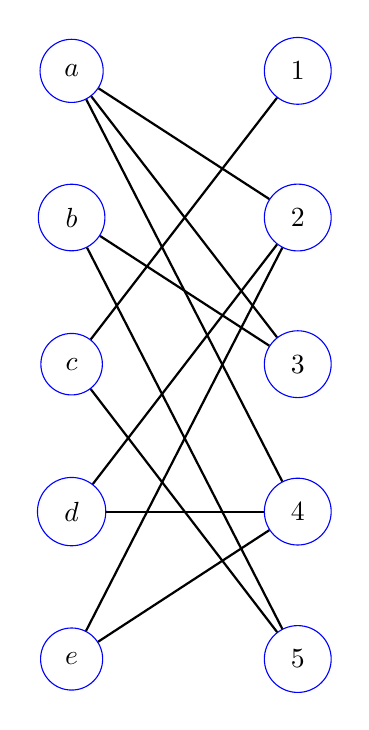
\begin{tikzpicture}[unmarked/.style={circle,inner sep=0.2cm,draw = blue}, edge/.style={thick}]
\matrix[row sep=1.0cm,column sep=2.0cm] 
{
\node(a)[unmarked]{$a$};  \pgfmatrixnextcell \node(1)[unmarked]{$1$};\\
\node(b)[unmarked]{$b$};  \pgfmatrixnextcell \node(2)[unmarked]{$2$};\\
\node(c)[unmarked]{$c$};  \pgfmatrixnextcell \node(3)[unmarked]{$3$};\\
\node(d)[unmarked]{$d$};  \pgfmatrixnextcell \node(4)[unmarked]{$4$};\\
\node(e)[unmarked]{$e$};  \pgfmatrixnextcell \node(5)[unmarked]{$5$};\\
};

\draw [edge] (a) to (2);
\draw [edge] (a) to (3);
\draw [edge] (a) to (4);
\draw [edge] (b) to (3);
\draw [edge] (b) to (5);
\draw [edge] (c) to (1);
\draw [edge] (c) to (5);
\draw [edge] (d) to (2);
\draw [edge] (d) to (4);
\draw [edge] (e) to (2);
\draw [edge] (e) to (4);
\end{tikzpicture}
\caption{Example of a bipartite graph}
\label{figure:bipartite}
\end{figure}

A common problem related to a bipartite graph is to find the largest \textbf{matching} $M$ in the graph; i.e. a subset $M\subseteq E$ of edges of $G$, no two of which share a common vertex.
Figure~\ref{figure:bipartite2} shows a matchiing for the graph in Figure~\ref{figure:bipartite}.

\begin{figure}
\centering
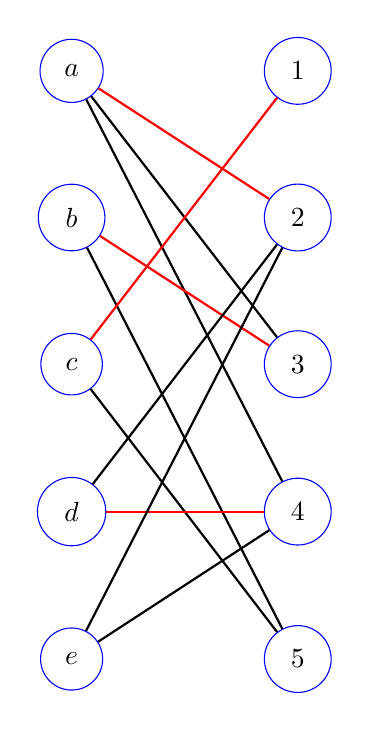
\begin{tikzpicture}[unmarked/.style={circle,inner sep=0.2cm,draw = blue}, edge/.style={thick},match/.style={thick,draw=red}]
\matrix[row sep=1.0cm,column sep=2.0cm] 
{
\node(a)[unmarked]{$a$};  \pgfmatrixnextcell \node(1)[unmarked]{$1$};\\
\node(b)[unmarked]{$b$};  \pgfmatrixnextcell \node(2)[unmarked]{$2$};\\
\node(c)[unmarked]{$c$};  \pgfmatrixnextcell \node(3)[unmarked]{$3$};\\
\node(d)[unmarked]{$d$};  \pgfmatrixnextcell \node(4)[unmarked]{$4$};\\
\node(e)[unmarked]{$e$};  \pgfmatrixnextcell \node(5)[unmarked]{$5$};\\
};

\draw [match] (a) to (2);
\draw [edge] (a) to (3);
\draw [edge] (a) to (4);
\draw [match] (b) to (3);
\draw [edge] (b) to (5);
\draw [match] (c) to (1);
\draw [edge] (c) to (5);
\draw [edge] (d) to (2);
\draw [match] (d) to (4);
\draw [edge] (e) to (2);
\draw [edge] (e) to (4);
\end{tikzpicture}
\caption{The red edges form a maximal matching for the bipartite graph.}
\label{figure:bipartite2}
\end{figure}

The following definitions prove useful when discussing matchings in a graph. Let $M$ be a matching.

\begin{description}
\item[Maximum Matching] $M$ is a called a {\bf maximum} matching
iff for any other matching $M^{\prime}$ of $G$, $|M^{\prime}|\leq |M|$.


\item[Maximal Matching] $M$ is called {\bf maximal} iff it is not contained in any larger matching. In other words, one cannot increase the size of $M$ simply by adding another edge to 
$M$.

\item[Matched and Free Edges] The edges of $M$ are called {\bf matched} edges while the edges in $E-M$ are called {\bf free} edges.

\item[Exposed and Covered Vertices] Any vertex that is not incident with an edge in $M$ is said to be {\bf exposed} by $M$.
otherwise it is {\bf covered} by $M$.

\item[Increment] Matching $M^{*}$ is called an \textbf{increment} of $M$ iff $|M^{*}|=|M|+1$
\end{description}

Notice that the matching $M$ in Figure~\ref{figure:bipartite2} is maximal, since no edge can be added to $M$ to increase its size. Indeed, the only exposed vertices are $e$ and $5$, but they are not adjacent.
However, $M$ is not a maximum matching. A maximum matching is shown in Figure~\ref{figure:bipartite3}. This matching is an increment of $M$

\begin{figure}
\centering
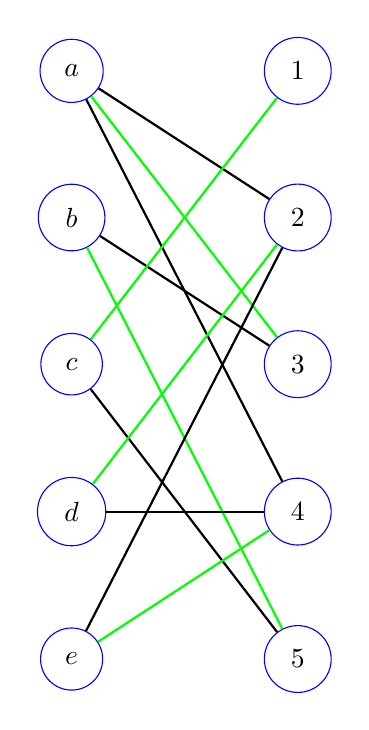
\begin{tikzpicture}[unmarked/.style={circle,inner sep=0.2cm,draw = blue}, edge/.style={thick},match/.style={thick,draw=green}]
\matrix[row sep=1.0cm,column sep=2.0cm] 
{
\node(a)[unmarked]{$a$};  \pgfmatrixnextcell \node(1)[unmarked]{$1$};\\
\node(b)[unmarked]{$b$};  \pgfmatrixnextcell \node(2)[unmarked]{$2$};\\
\node(c)[unmarked]{$c$};  \pgfmatrixnextcell \node(3)[unmarked]{$3$};\\
\node(d)[unmarked]{$d$};  \pgfmatrixnextcell \node(4)[unmarked]{$4$};\\
\node(e)[unmarked]{$e$};  \pgfmatrixnextcell \node(5)[unmarked]{$5$};\\
};

\draw [match] (a) to (3);
\draw [edge] (a) to (2);
\draw [edge] (a) to (4);
\draw [match] (b) to (5);
\draw [edge] (b) to (3);
\draw [match] (c) to (1);
\draw [edge] (c) to (5);
\draw [edge] (d) to (4);
\draw [match] (d) to (2);
\draw [edge] (e) to (2);
\draw [match] (e) to (4);
\end{tikzpicture}
\caption{The green edges form a maximum matching for the bipartite graph.}
\label{figure:bipartite3}
\end{figure}

We now describe method for transforming a non-maximum maximal matching $M$ of $G=(V,E)$ into a matching $M^{\prime}$ that has one more edge than $M$. 
The first step is to construct the \textbf{flow graph} $F_{G,M}$ with respect to $G$ and $M$. This graph is a directed graph whose vertices are the vertices of $G$ with two 
additional vertices $s$ and $t$, the \textbf{source} and \textbf{destination} vertices, respectively. Moreover, the edges of $F_{G,M}$ are defined as follows. Note: for each 
$(u,v)\in E$, we assume $u\in V_{\mbox{left}}$ and  $v\in V_{\mbox{right}}$.

\begin{enumerate}
\item For $(u,v)\in E$, if $(u,v)\not\in M$, then $(u,v)$ is an edge of $F_{G,M}$. This edge is oriented ``left-to-right''.
\item For $(u,v)\in E$, if $(u,v)\in M$, then $(v,u)$ is an edge of $F_{G,M}$. This edge is oriented ``right-to-left''.
\item For $u\in V_{\mbox{left}}$, if $u$ is exposed, then $(s,u)$ is an edge of $F_{G,M}$. This edge is oriented ``left-to-right''.
\item For $u\in V_{\mbox{left}}$, if $u$ is covered, then $(u,s)$ is an edge of $F_{G,M}$. This edge is oriented  ``right-to-left''.
\item For $v\in V_{\mbox{right}}$, if $v$ is exposed, then $(v,t)$ is an edge of $F_{G,M}$. This edge is oriented ``left-to-right''.
\item For $v\in V_{\mbox{right}}$, if $v$ is covered, then $(t,v)$ is an edge of $F_{G,M}$. This edge is oriented  ``right-to-left''.
\end{enumerate}

Figure~\ref{figure:bipartite4} shows $F_{G,M}$ for the graph $G$ and matching $M$ from Figure~\ref{figure:bipartite2}.

\begin{figure}
\centering
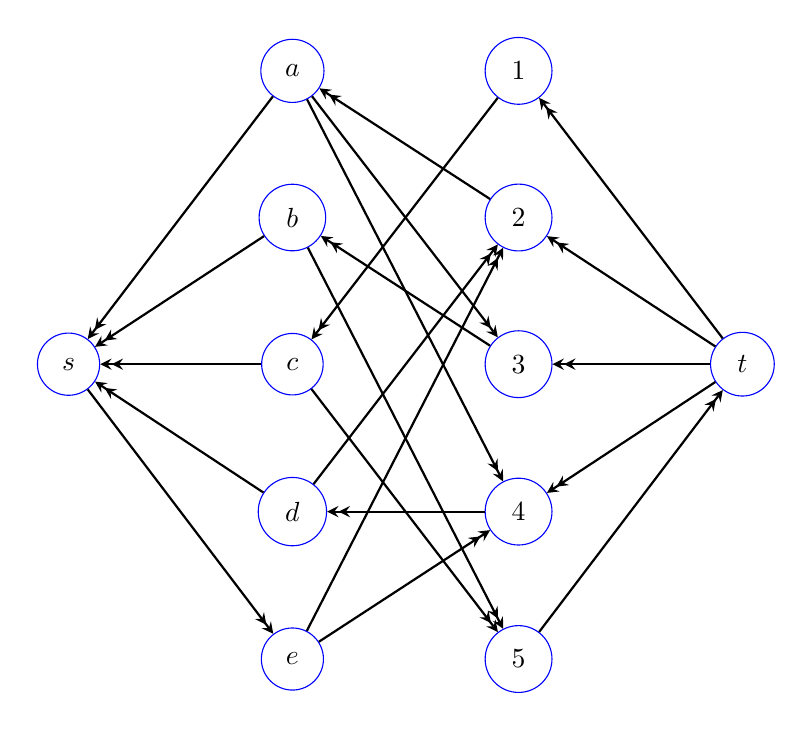
\begin{tikzpicture}[unmarked/.style={circle,inner sep=0.2cm,draw = blue}, edge/.style={thick,->>,>=stealth},blank/.style={}]
\matrix[row sep=1.0cm,column sep=2.0cm] 
{
\node()[blank]{};  \pgfmatrixnextcell \node(a)[unmarked]{$a$};  \pgfmatrixnextcell \node(1)[unmarked]{$1$};  \pgfmatrixnextcell \node()[blank]{};\\
\node()[blank]{};  \pgfmatrixnextcell \node(b)[unmarked]{$b$};  \pgfmatrixnextcell \node(2)[unmarked]{$2$};  \pgfmatrixnextcell \node()[blank]{};\\
\node(s)[unmarked]{$s$};  \pgfmatrixnextcell \node(c)[unmarked]{$c$};  \pgfmatrixnextcell \node(3)[unmarked]{$3$};  \pgfmatrixnextcell \node(t)[unmarked]{$t$};\\
\node()[blank]{};  \pgfmatrixnextcell \node(d)[unmarked]{$d$};  \pgfmatrixnextcell \node(4)[unmarked]{$4$};  \pgfmatrixnextcell \node()[blank]{};\\
\node()[blank]{};  \pgfmatrixnextcell \node(e)[unmarked]{$e$};  \pgfmatrixnextcell \node(5)[unmarked]{$5$};  \pgfmatrixnextcell \node()[blank]{};\\
};

\draw [edge] (2) to (a);
\draw [edge] (a) to (3);
\draw [edge] (a) to (4);
\draw [edge] (3) to (b);
\draw [edge] (b) to (5);
\draw [edge] (1) to (c);
\draw [edge] (c) to (5);
\draw [edge] (d) to (2);
\draw [edge] (4) to (d);
\draw [edge] (e) to (2);
\draw [edge] (e) to (4);
\draw [edge] (a) to (s);
\draw [edge] (b) to (s);
\draw [edge] (c) to (s);
\draw [edge] (d) to (s);
\draw [edge] (s) to (e);
\draw [edge] (t) to (1);
\draw [edge] (t) to (2);
\draw [edge] (t) to (3);
\draw [edge] (t) to (4);
\draw [edge] (5) to (t);
\end{tikzpicture}
\caption{$F_{G,M}$ for the graph $G$ and matching $M$ of Figure 2.}
\label{figure:bipartite4}
\end{figure}

Notice that any simple path $P$ from $s$ to $t$ in $F_{G,M}$ starts with an edge $(s,a)$, and ends with an edge $(b,t)$, where $a$ and $b$ are exposed vertices.
The part of $P$ that starts at $a$ and ends at $b$ is called an \textbf{alternating path} of $F_{G,M}$. 
Figure~\ref{figure:bipartite5} shows an alternating path for the flow graph $F_{G,M}$  from Figure~\ref{figure:bipartite4}.

\begin{figure}
\centering
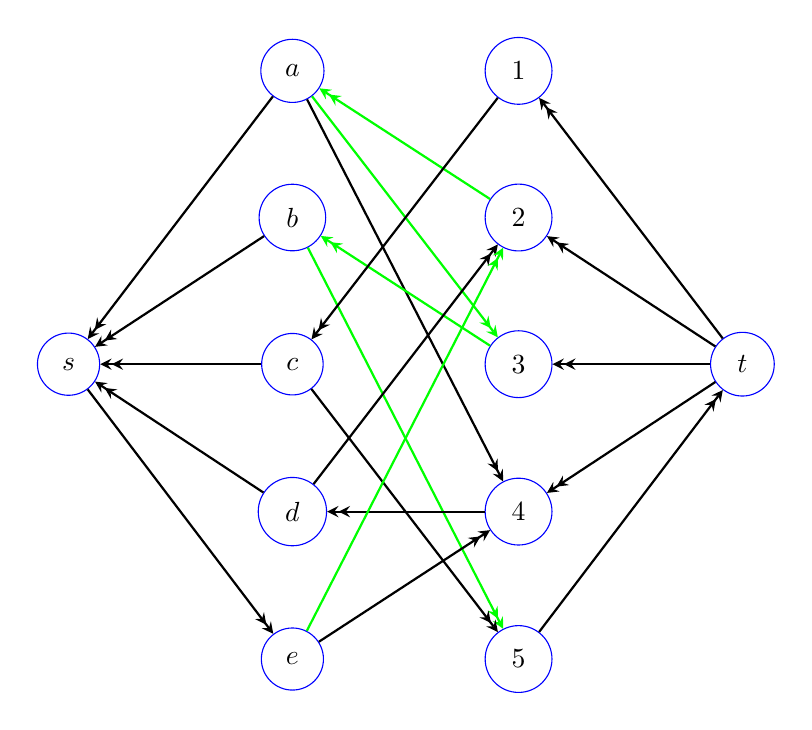
\begin{tikzpicture}[unmarked/.style={circle,inner sep=0.2cm,draw = blue}, edge/.style={thick,->>,>=stealth},blank/.style={},alternate/.style={thick,->>,draw=green,>=stealth}]
\matrix[row sep=1.0cm,column sep=2.0cm] 
{
\node()[blank]{};  \pgfmatrixnextcell \node(a)[unmarked]{$a$};  \pgfmatrixnextcell \node(1)[unmarked]{$1$};  \pgfmatrixnextcell \node()[blank]{};\\
\node()[blank]{};  \pgfmatrixnextcell \node(b)[unmarked]{$b$};  \pgfmatrixnextcell \node(2)[unmarked]{$2$};  \pgfmatrixnextcell \node()[blank]{};\\
\node(s)[unmarked]{$s$};  \pgfmatrixnextcell \node(c)[unmarked]{$c$};  \pgfmatrixnextcell \node(3)[unmarked]{$3$};  \pgfmatrixnextcell \node(t)[unmarked]{$t$};\\
\node()[blank]{};  \pgfmatrixnextcell \node(d)[unmarked]{$d$};  \pgfmatrixnextcell \node(4)[unmarked]{$4$};  \pgfmatrixnextcell \node()[blank]{};\\
\node()[blank]{};  \pgfmatrixnextcell \node(e)[unmarked]{$e$};  \pgfmatrixnextcell \node(5)[unmarked]{$5$};  \pgfmatrixnextcell \node()[blank]{};\\
};

\draw [alternate] (2) to (a);
\draw [alternate] (a) to (3);
\draw [edge] (a) to (4);
\draw [alternate] (3) to (b);
\draw [alternate] (b) to (5);
\draw [edge] (1) to (c);
\draw [edge] (c) to (5);
\draw [edge] (d) to (2);
\draw [edge] (4) to (d);
\draw [alternate] (e) to (2);
\draw [edge] (e) to (4);
\draw [edge] (a) to (s);
\draw [edge] (b) to (s);
\draw [edge] (c) to (s);
\draw [edge] (d) to (s);
\draw [edge] (s) to (e);
\draw [edge] (t) to (1);
\draw [edge] (t) to (2);
\draw [edge] (t) to (3);
\draw [edge] (t) to (4);
\draw [edge] (5) to (t);
\end{tikzpicture}
\caption{Alternating path (in green) for flow graph $F_{G,M}$ of Figure 4.}
\label{figure:bipartite5}
\end{figure}

Finally, the set operation $A\oplus B$ is called the \textbf{symmetric difference}
between $A$ and $B$ and consists of all elements that are either in $A$ but not $B$, or in $B$ but not $A$. The value $|A\oplus B|$ is often referred to as a \textbf{similarity measure}, where 
 $|A\oplus B|$ will be smaller for sets that are more similar. For example, $|A\oplus A|=0$, and so $A$ is the set that is most similar to $A$ (obviously!).

{\bf Lemma 1.} Let $G$ be a bipartite graph and $M$ a matching in $G$. Then if $P$ is an alternating path in $F_{G,M}$, then $M^{*}=P\oplus M$ is an increment of $M$.

{\bf Proof of Lemma 1.} Assume $G$ be a bipartite graph, $M$ a matching in $G$, and $P$ is an alternating path in $F_{G,M}$. 
 Let $P_{\mbox{left}}$ denote $P$'s left-to-right edges, and $P_{\mbox{right}}$ denote
its right-to-left edges. Then $P_{\mbox{left}}$ consists of the odd edges of $P$, while $P_{\mbox{right}}$ consists of $P$'s even edges. Also,
since an alternating path begins on the left side, and ends on the
right side, we must have  $|P_{\mbox{left}}|=|P_{\mbox{right}}|+1$. Next, notice that both $P_{\mbox{left}}$ and $P_{\mbox{right}}$ are matchings of $G$.  $P_{\mbox{right}}$ is certainly   a
matching, since it is  a subset of $M$, while $P_{\mbox{left}}$ is a matching since $P$ is simple, and no two edges of  $P_{\mbox{left}}$ occur in succession within $P$, and hence do not share any vertices.

Finally, notice that 
\[P\oplus M=P_{\mbox{left}}\cup (M-P_{\mbox{right}}),\]
and so $|P\oplus M|=|M|+1$. 
It remains to show that $P\oplus M$ is a matching. Since $P_{\mbox{left}}$ and $M-P_{\mbox{right}}$ are both matchings, their union will be a matching provided no edge of 
$P_{\mbox{left}}$ shares a vertex with some edge of  $M-P_{\mbox{right}}$. But a vertex of any edge in $P_{\mbox{left}}$ is either exposed, or is shared with an edge in $P_{\mbox{right}}$, and hence
cannot be shared with an edge in $M-P_{\mbox{right}}$, since $P_{\mbox{right}}\cup M-P_{\mbox{right}}=M$ is a matching. 
Therefore, $M^{*}=P\oplus M$ is an increment of $M$.

It turns out that the converse of Lemma 1 is also true.

{\bf Theorem 2.} If matching $M$ of bipartite graph $G$ has an increment, then  $F_{G,M}$ has an alternating path.

{\bf Proof of Theorem 2.} Suppose matching $M$ of bipartite graph $G$ has an increment. Let  $M^{*}$ be the increment of $M$ that is most similar to $M$; i.e. 
$|M^{*}\oplus M|$ is a minimum over all possible increments of $M$. We make the following two claims about $M^{*}$.

\begin{enumerate}
\item $M^{*}$ covers exactly two vertices that are exposed by $M$, one in $V_{\mbox{left}}$ and the other in $V_{\mbox{right}}$.
\item $M^{*}\oplus M$ is an alternating path of  $F_{G,M}$.
\end{enumerate}

The proof is by induction on $|M^{*}\oplus M|$.

\textbf{Basis Step.} Assume $|M^{*}\oplus M|=1$. In this case, since  $|M^{*}|=|M|+1$, it follows that $M^{*}=M+(a,b)$, where $a$ and $b$ are exposed by $M$. Hence, $P=a,b$ is an alternating path
of  $F_{G,M}$, with $P=M^{*}\oplus M$. Moreover, $a\in V_{\mbox{left}}$ and $b\in V_{\mbox{right}}$ are the only vertices that are exposed by $M$ and covered by $M^{*}$.

\textbf{Inductive Step.}  Assume the two claims are true for any graph $G$ and matching $M$ for which $|M^{*}\oplus M| \leq k-1$, for some $k\geq 2$. Now assume 
 $|M^{*}\oplus M| = k\geq 2$. Let $a\in V_{\mbox{left}}$ be a vertex that is exposed by $M$, but covered by $M^{*}$ via edge $(a,v)$. Then there is some edge $(u,v)\in M$ that shares vertex $v$ with $(a,v)$.
 Otherwise, $M^{\prime}=M+(a,v)$ would be an increment of $M$ for which  $|M^{\prime}\oplus M|=1$, contradicting the assumption that $M^{*}$ is the most similar increment of $M$. Also, there must
 be an edge $(u,v_2)\in M^{*}$. Otherwise, $M^{\prime}=M^{*}-(a,v)+(u,v)$ is an increment of $M$ for which $|M^{\prime}\oplus M|=|M^{*}\oplus M|-2$, which implies another contradiction.
 
Now let $G^{\prime}$ be the bipartite graph that results in removing vertices $a$ and $v$ from $G$, as well as all edges that are incident with these vertices. Then $M-(u,v)$ is a matching in  $G^{\prime}$. Notice also that $M^{*}-(a,v)$ is also a matching in $G^{\prime}$ with  
\[|M^{*}-(a,v)| = |M^{*}|-1 = |M| = |M-(u,v)| + 1,\]
and is thus
an increment of 
 $M-(u,v)$ in $G^{\prime}$.
 
\textbf{Claim.} $M^{*}-(a,v)$ is the increment of  $M-(u,v)$ that is most similar to  $M-(u,v)$. Suppose otherwise. Let $M^{\prime}$ be a matching of $G^{\prime}$ that is the most similar increment of
 $M-(u,v)$. Then $M^{\prime}+(a,v)$ is an increment of $M$ in $G$ with
 \[|M^{\prime}+(a,v)\oplus M| = |M^{\prime}\oplus M-(u,v)| + 2 <  |M^{*}-(a,v)\oplus M-(u,v)| + 2 = |M^{*}\oplus M|,\]
 where the inequality stems from the assumption that  $M^{\prime}$ is more similar to  $M-(u,v)$ than is $M^{*}-(a,v)$. But this leads to a contradiction, since it implies 
 $M^{\prime}+(a,v)$ is more similar to $M$ than $M^{*}$ in $G$. Hence,  $M^{*}-(a,v)$ is the most similar increment of  $M-(u,v)$  in $G^{\prime}$.
 
 Now since  \[|M^{*}-(a,v)\oplus M-(u,v)|=|M^{*}\oplus M|-2=k-2 < k-1,\]
 by the inductive assumption, $M^{*}-(a,v)$ covers exactly two vertices that are exposed by $M-(u,v)$ in $G^{\prime}$. And since $(u,v_2)\in M^{*}$ it follws that one of the vertices is $u\in V_{\mbox{left}}$, while
 the other is some vertex $b\in V_{\mbox{right}}$. Moreover, letting $F^{\prime}$ be the flow graph with respect to $G^{\prime}$ and matching $M-(u,v)$, the inductive assumption implies that 
  $M^{*}-(a,v)\oplus M-(u,v)$ is an alternating path in  $F^{\prime}$. And this path begins at $u$ and ends at $b$. Therefore, by prepending the edges $(a,v)$ and $(v,u)=(u,v)$ to this path, we see that
 $M^{*}\oplus M$ is an alternating path in $F_{G,M}$ from $M$-exposed vertex $a\in  V_{\mbox{left}}$ to  $M$-exposed vertex $b\in V_{\mbox{right}}$. 
 Moreover, these are the only $M$-exposed vertices covered by $M^{*}$.
 
Theorem 2 implies the following algorithm for finding a maximum matching within a bipartite graph $G$.

\subsection*{Maximum Matching Algorithm}
\begin{itemize}
 \renewcommand{\labelitemi}{}
 \renewcommand{\labelitemii}{}
 \renewcommand{\labelitemiii}{}
\item Input bipartite graph $G$.
\item Initialize matching $M$: $M\leftarrow\emptyset$.
\item While there is a vertex of $G$ that is exposed by $M$
\begin{itemize}
\item If $F_{G,M}$ has no alternating path, then return $M$.
\item Let $P$ be an alternating path of  $F_{G,M}$.
\item Update $M$: $M\leftarrow P\oplus M$.
\end{itemize}
\item Return $M$.
\end{itemize}

The \textbf{Perfect Matching} decision problem is the problem of deciding if a bitpartite graph $G$ has a \textbf{perfect mathching}, i.e. one that covers every vertex of $G$. 
Theorem 2 implies the following corollary. For a bipartite graph to have such a matching, it must be the case that $|V_{\mbox{left}}|=|V_{\mbox{right}}|$.

{\bf Corollary 2.} The Perfect Matching decision problem is polynomial-time Turing reducible to Reachability, while requiring at most $n$ queries, where $n=|V_{\mbox{left}}|=|V_{\mbox{right}}|$.
Moreover, each query can be answered in $\mbox{O}(m+n)$ steps, where $m$ is the number of edges of $G$. Assuming $m > n$, this yields a running time of $T(m,n)=\mbox{O}(nm)$ for the 
Perfect Matching algorithm. 








\newpage
\section*{Exercises}

\begin{enumerate}

\item Does Johnny's algorithm from Example 1 prove that Multioly is polynomial-time Turing reducible to Add? Explain.

\item Prove that the $\leq_{\mbox{T}}^{\mbox{p}}$ is transitive. In other words, if $L_{1}\leq_{\mbox{T}}^{\mbox{p}}L_{2}$ and
$L_{2}\leq_{\mbox{T}}^{\mbox{p}}L_{3}$, then $L_{1}\leq_{\mbox{T}}^{\mbox{p}}L_{3}$.


\item Given Boolean function $F(x_{1},x_{2},x_{3},x_{4})=$
\[
(x_{1}\vee \overline{x}_{3}\vee x_{4})\wedge
(\overline{x}_{1}\vee \overline{x}_{3}\vee x_{4})\wedge
(\overline{x}_{1}\vee(\overline{x}_{2}\wedge x_{3}))\wedge
(\overline{x}_{1}\wedge(x_{2}\vee\overline{x}_{4}))\wedge
(\overline{x}_{1}\wedge x_{2}\wedge x_{4}),
\]
evaluate $F(a)$ for $a=(1,1,1,1)$. Is $F$ satisfiable? If so, provide
a satisfying assignment for $F$.

\item Provide a Boolean formula that is logically equivalent to the defining formula
from the previous problem, but is in conjunctive normal form. For what value of $k$ is this
 formula an instance of the
k-CNF-SAT problem?

\item For the directed graph
$G=(V,E)$, where \[V=\{a,b,c,d,e,f,g,h,i,j,k\}\] and the edges are given by
\[E=\{(a,b),(a,c),(b,c),(b,d),(b,e),(b,g),(c,g),(c,f),\] 
\[(d,f),(f,g),(f,h),(g,h),(i,j),(i,k),(j,k)\},\]
use the Reachability Algorithm to determine if vertex $k$ is reachable from vertex $a$.
Show the contents of the FIFO queue $Q$ at each stage of the algorithm.

\item Re-write the CNF formula from Problem 2 in CNF notation.

\item Draw the implication graph for the following set of CNF clauses.
\[
(\overline{x}_{2},\overline{x}_{3}),
(x_{2},\overline{x}_{4}),
(x_{1},\overline{x}_{3}),
(x_{2},x_{3}),
(x_{1},x_{4}),
(\overline{x}_{1},x_{4}),
(x_{1},\overline{x}_{2}).\]
Perform the 2SAT Algorithm to determine a satisfying assignment for this set of clauses.

\item Repeat the previous problem, but now add the additional clause $(\overline{x}_{2},x_{3})$.
Verify that there is now a cycle in the implication graph which contains a variable and its negation.
Which variable is it?


\item For bipartite graph $G=(U,V,E)$ we have $U=\{u_{1},u_{2},u_{3},u_{4}\}$, $V=\{v_{1},v_{2},v_{3},v_{4}\}$, and 
\[E=\{(u_{1},v_{1}),(u_{1},v_{2}),(u_{1},v_{4}),(u_{2},v_{1}),(u_{2},v_{3}),\]
\[(u_{2},v_{4}),(u_{3},v_{1}),(u_{3},v_{3}),(u_{4},v_{1}),(u_{4},v_{3})\}.\]

\begin{enumerate}
\item Draw $G$.
\item Does $G$ have a (non-maximum) maximal matching $M$ of size 1? size 2? size 3? 
\item For each ``yes'' answer to the previous part, draw the flow graph $F_{G,M}$ associated with the 
matching, and provide an alternating path $P$ in  $F_{G,M}$. Use the alternating path to find an increment of $M$.
\end{enumerate}


\item At a school ice-cream party there are five dixie cups of ice cream that remain to be served. Each cup 
has a different flavor: vanilla, chocolate, cherry, rocky road, and mint and chip. There are five children
who have yet to be served: Abe, Ben, Cris, Dan, and Eva. The ice-cream preferences of these children are shown below.

\vspace{0.25in}
\begin{tabular}{|l|ccccc|}
\hline
\textbf{Child} & \textbf{Vanilla} & \textbf{Chocolate} & \textbf{Cherry} & \textbf{Rocky Road} & 
\textbf{Mint \& Chip}\\
\hline
Abe & X & & X & & X\\
Ben &  & X &  & & \\
Cris &  & X &  & X & \\
Dan &  & X &  & & X\\
Eva &  &  & X & X & \\
\hline
\end{tabular}

\vspace{0.25in}
In a rush to get their ice cream, Abe grabbed the cherry, Cris the chocolate, Dan the mint and chip, and 
Eva the rocky road. This left Ben with a (vanilla) flavor that he does not like, and which he refused to eat.
Show how the maximum-matching algorithm can be used to increase the current matching (of four children to four
ice creams that they prefer) to a matching of size five, in which each child will be assigned an ice cream that
he or she prefers.

\item Prove that, for any three sets $A$, $B$, and $C$. $|A\oplus B|\leq |A\oplus C| + |C\oplus B|$.





\end{enumerate}

\newpage
\newpage
\section*{Exercise Solutions}

\begin{enumerate}
\item Johnny's algorithm does \textit{not} run in polynomial time. To see this, suppose that Johny wants the answer to $m\times m$. Then 
the the size of this problem instance is $2\lfloor\log m\rfloor$. However, Johnny's algorithm will require the $m-1$ queries 
\[m+m, 2m+m, \ldots, (m-1)m+m,\]
and $m-1$ is exponential with respect to $\log m$. Thus, the number of algorithm steps grows exponentially with respect to the problem size.

\item Suppose $L_{1}\leq_{\mbox{T}}^{\mbox{p}}L_{2}$. Then there is a polynomial $p(n)$ and an algorithm $A_{12}$ that solves a size-$n$ instance of 
$L_{1}$ by making at most $p(n)$ queries to $L_{2}$. Moreover, since  $L_{2}\leq_{\mbox{T}}^{\mbox{p}}L_{3}$, 
there is also a polynomial $q(m)$, and an algorithm $A_{23}$ that solves each size-$m$ instance of $L_{2}$ by making
at most $q(m)$ queries to $L_{3}$. 

We now describe an algorithm $A_{13}$ for polynomial-time reducing $L_{1}$ to $L_{3}$. 
This algorithm  is obtained by taking $A_{12}$ and modifying it
as follows. For each query step $\mbox{query}(y)$, where $y$ is an instance of $L_{2}$, we replace this step with $A_{23}(y)$, which is the answer returned by $A_{23}$ on input $y$.
We may think of $A_{23}(y)$ as a function call that is being made within the body of $A_{13}$. Of course, the $A_{23}$ function has its own body of source code, which is now part of the $A_{13}$ code base.
After modifying $A_{12}$ in this manner to obtain $A_{13}$, notice that the only query steps in  $A_{13}$ are found in the $A_{23}$ code, and are of the form $\mbox{query}(z)$, where
$z$ is a problem instance of $L_{3}$. Hence, $A_{13}$ is an algorithm that Turing reduces $L_{1}$ to $L_{3}$. It only remains to show that $A_{13}$ runs in time polynomial in $n$.
To see this, first note that the non-query steps of  $A_{13}$ are the same non-query steps as $A_{12}$, and that the number of such steps is bounded by $p(n)$. Also, since $A_{12}$ makes at most
$p(n)$ queries (why?) to $L_{2}$, it follows that  $A_{13}$ calls the $A_{23}$ function at most $p(n)$ times. Moreover, the running time of each function call $A_{23}(y)$ is bounded by $q(m)$, where
$m$ is the size of $L_{2}$-problem $y$. But this size is bounded by $p(n)$, since $p(n)$ is the maximum number of allowable steps that can be made to construct an $L_{2}$ query, and we assume that
it takes a single algorithm step to construct a single bit of $y$. Thus, each function call to $A_{23}$ will have a running time that is bounded by $q(p(n))$, which is a polynomial, since the compostion of 
two polynomials is also a polynomial.  Finally, since there are at most $p(n)$ function calls to $A_{23}$ it follows that the total running time due to the function calls is 
bounded by the polynomial  $p(n)q(p(n))$, and so $A_{13}$ has running time $\mbox{O}(p(n)q(p(n)))$. Therefore, $L_{1}\leq_{\mbox{T}}^{\mbox{p}}L_{3}$.


\item $F(1,1,1,1)=0$. $F$ is satisfied by $a=(0,1,0,1)$.

\item 
\[
(x_{1}\vee \overline{x}_{3}\vee x_{4})\wedge
(\overline{x}_{1}\vee \overline{x}_{3}\vee x_{4})\wedge
(\overline{x}_{1}\vee\overline{x}_{2})\wedge
(\overline{x}_{1}\vee x_{3})\wedge
\overline{x}_{1}\wedge(x_{2}\vee\overline{x}_{4})\wedge
\overline{x}_{1}\wedge x_{2}\wedge x_{4}.
\]


\item Queue sequence: $Q_{1}=\{a\}$, $Q_{2}=\{b,c\}$, $Q_{3}=\{c,d,e,g\}$, $Q_{4}=\{d,e,g,f\}$, $Q_{5}=\{e,g,f\}$, $Q_{6}=\{g,f\}$, $Q_{7}=\{f,h\}$, 
$Q_{8}=\{h\}$, $Q_{9}=\emptyset$. Therefore, vertex $k$ is not reachable from $a$.

\item 
\[\mathcal{C}=\{(x_{1},\overline{x}_{3},x_{4}),
(\overline{x}_{1}, \overline{x}_{3}, x_{4}),
(\overline{x}_{1},\overline{x}_{2}),
(\overline{x}_{1}, x_{3}),
(\overline{x}_{1}),(x_{2},\overline{x}_{4}),
(\overline{x}_{1}), (x_{2}), (x_{4})\}
\]

\item  See $G_{\mathcal{C}}$ above.

\begin{figure}
\centering
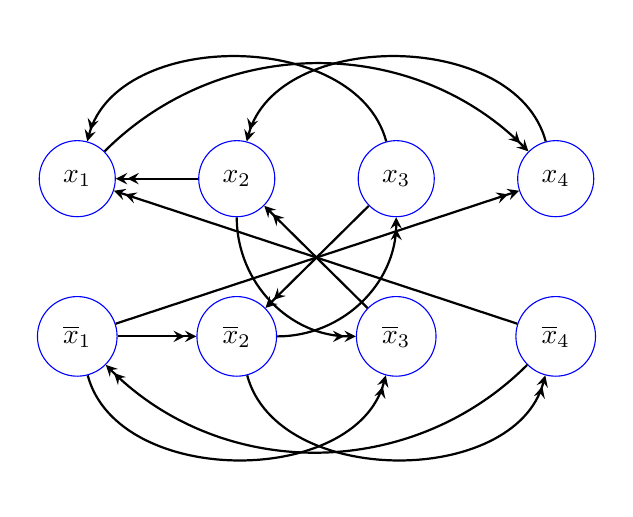
\begin{tikzpicture}[unmarked/.style={circle,inner sep=0.2cm,draw = blue}, edge/.style={thick,->>,>=stealth}]
\matrix[row sep=1.0cm,column sep=1.0cm] 
{
\node(x1)[unmarked]{$x_{1}$};  \pgfmatrixnextcell \node(x2)[unmarked]{$x_{2}$};  \pgfmatrixnextcell \node(x3)[unmarked]{$x_{3}$}; \pgfmatrixnextcell \node(x4)[unmarked]{$x_{4}$};\\
\node(nx1)[unmarked]{$\overline{x}_{1}$};  \pgfmatrixnextcell \node(nx2)[unmarked]{$\overline{x}_{2}$};  \pgfmatrixnextcell \node(nx3)[unmarked]{$\overline{x}_{3}$}; 
\pgfmatrixnextcell \node(nx4)[unmarked]{$\overline{x}_{4}$};\\
};
%\draw[edge](a)--(b);\draw[edge](b)--(c);\draw[edge](a)--(d);\draw[edge](b)--(e);\draw[edge](c)--(f);\draw[edge](d)--(e);\draw[edge](e)--(f);\draw[edge](d)--(h);\draw[edge](e)--(g);
%\draw[edge](f)--(i);\draw[edge](h)--(g);\draw[edge](g)--(i);\draw[edge](h)--(e);\draw[edge](b)--(f);
\draw [edge] (nx4) to [bend left=45] (nx1);
\draw [edge] (nx4) to (x1);
\draw [edge] (nx2) to [bend right=75] (nx4);
\draw [edge] (x4) to [bend right=75] (x2);
\draw [edge] (nx1) to [bend right=75] (nx3);
\draw [edge] (nx3) to (x2);
\draw [edge] (x2) to [out=270,in=180] (nx3);
\draw [edge] (nx1) to (nx2);
\draw [edge] (x2) to (x1);
\draw [edge] (nx2) to [out=0,in=270] (x3);
\draw [edge] (x3) to (nx2);
\draw [edge] (nx1) to (x4);
\draw [edge] (x1) to [bend left=45] (x4);
\draw [edge] (x3) to [bend right=75] (x1);
\end{tikzpicture}
\caption{Exercise 5:$G_{\mathcal{C}}$}
\end{figure}

\begin{tabular}{|l|l|l|}
\hline
\textbf{Round} & \textbf{Root Vertex} & \textbf{Reachable Set $R$}\\
\hline
1 & $x_{1}$ & $R=\{x_{1},x_{2},\overline{x}_{3},x_{4}\}$\\
\hline
\end{tabular}

\item See Figure 2 above.
\begin{figure}
\centering
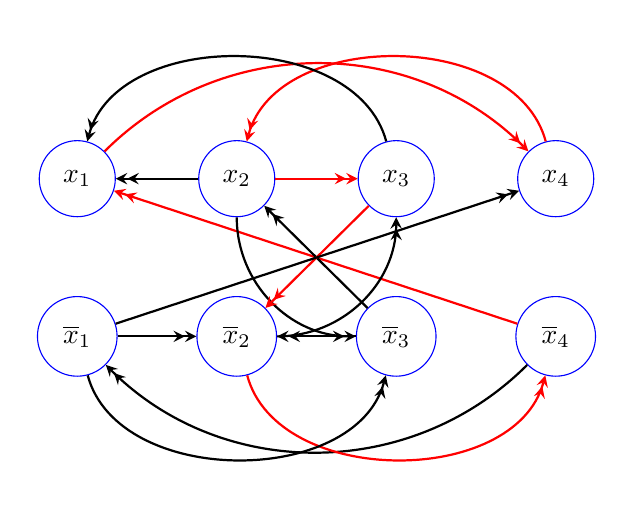
\begin{tikzpicture}[unmarked/.style={circle,inner sep=0.2cm,draw = blue}, edge/.style={thick,->>,>=stealth},cycle_edge/.style={thick,->>,draw=red,>=stealth}]
\matrix[row sep=1.0cm,column sep=1.0cm] 
{
\node(x1)[unmarked]{$x_{1}$};  \pgfmatrixnextcell \node(x2)[unmarked]{$x_{2}$};  \pgfmatrixnextcell \node(x3)[unmarked]{$x_{3}$}; \pgfmatrixnextcell \node(x4)[unmarked]{$x_{4}$};\\
\node(nx1)[unmarked]{$\overline{x}_{1}$};  \pgfmatrixnextcell \node(nx2)[unmarked]{$\overline{x}_{2}$};  \pgfmatrixnextcell \node(nx3)[unmarked]{$\overline{x}_{3}$}; 
\pgfmatrixnextcell \node(nx4)[unmarked]{$\overline{x}_{4}$};\\
};
%\draw[edge](a)--(b);\draw[edge](b)--(c);\draw[edge](a)--(d);\draw[edge](b)--(e);\draw[edge](c)--(f);\draw[edge](d)--(e);\draw[edge](e)--(f);\draw[edge](d)--(h);\draw[edge](e)--(g);
%\draw[edge](f)--(i);\draw[edge](h)--(g);\draw[edge](g)--(i);\draw[edge](h)--(e);\draw[edge](b)--(f);
\draw [edge] (nx4) to [bend left=45] (nx1);
\draw [cycle_edge] (nx4) to (x1);
\draw [cycle_edge] (nx2) to [bend right=75] (nx4);
\draw [cycle_edge] (x4) to [bend right=75] (x2);
\draw [edge] (nx1) to [bend right=75] (nx3);
\draw [edge] (nx3) to (x2);
\draw [edge] (x2) to [out=270,in=180] (nx3);
\draw [edge] (nx1) to (nx2);
\draw [edge] (x2) to (x1);
\draw [edge] (nx2) to [out=0,in=270] (x3);
\draw [cycle_edge] (x3) to (nx2);
\draw [edge] (nx1) to (x4);
\draw [cycle_edge] (x1) to [bend left=45] (x4);
\draw [edge] (x3) to [bend right=75] (x1);
\draw [cycle_edge] (x2) to (x3);
\draw [edge] (nx3) to (nx2);
\end{tikzpicture}
\caption{Exercise 6: $G_{\mathcal{C}}$ and a ``bad'' cycle (in red)}
\end{figure}

\item 
\begin{enumerate}
\item Below is a graph of $G=(U,V,E)$

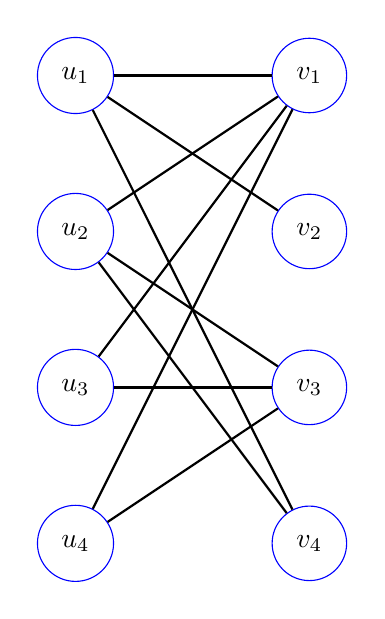
\begin{tikzpicture}[unmarked/.style={circle,inner sep=0.2cm,draw = blue}, edge/.style={thick}]
\matrix[row sep=1.0cm,column sep=2.0cm] 
{
\node(u1)[unmarked]{$u_1$};  \pgfmatrixnextcell \node(v1)[unmarked]{$v_1$};\\
\node(u2)[unmarked]{$u_2$};  \pgfmatrixnextcell \node(v2)[unmarked]{$v_2$};\\
\node(u3)[unmarked]{$u_3$};  \pgfmatrixnextcell \node(v3)[unmarked]{$v_3$};\\
\node(u4)[unmarked]{$u_4$};  \pgfmatrixnextcell \node(v4)[unmarked]{$v_4$};\\
};

\draw [edge] (u1) to (v1);
\draw [edge] (u1) to (v2);
\draw [edge] (u1) to (v4);
\draw [edge] (u2) to (v1);
\draw [edge] (u2) to (v3);
\draw [edge] (u2) to (v4);
\draw [edge] (u3) to (v1);
\draw [edge] (u3) to (v3);
\draw [edge] (u4) to (v1);
\draw [edge] (u4) to (v3);
\end{tikzpicture}

\item $G$ does not have a size-1 maximal matching since, for any edge $e$, there is an edge $e_{2}$ that does not share any vertices with $e$.
However, $M_2=\{(u_{1},v_{1}),(u_{2},v_{3})\}$ is a maximal matching of size 2, since $u_1$ and $u_2$ are the only vertices incident with $v_2$ and $v_{4}$.
Then $P=u_4,v_1,u_1,v_4$ is an alternating path in $F_{G,M_{2}}$, and $M_{3}=P\oplus M_{2}=\{(u_1,v_4),(u_4,v_1),(u_2,v_3)\}$ is a maximal matching of size 3.

\item $F_{G,M_{2}}$ is shown below with an alternating path $P$ drawn in green. This yields increment $M_{3}=P\oplus M_{2}=\{(u_1,v_4),(u_4,v_1),(u_2,v_3)\}$.

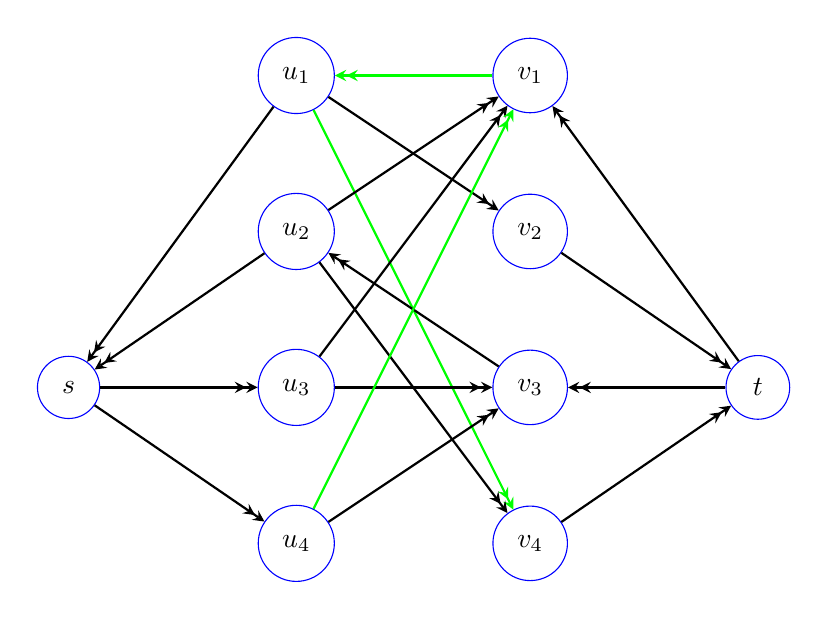
\begin{tikzpicture}[unmarked/.style={circle,inner sep=0.2cm,draw = blue}, edge/.style={thick,->>,>=stealth},blank/.style={},alternate/.style={thick,->>,draw=green,>=stealth}]
\matrix[row sep=1.0cm,column sep=2.0cm] 
{
\node()[blank]{};  \pgfmatrixnextcell \node(u1)[unmarked]{$u_1$};  \pgfmatrixnextcell \node(v1)[unmarked]{$v_1$};  \pgfmatrixnextcell \node()[blank]{};\\
\node()[blank]{};  \pgfmatrixnextcell \node(u2)[unmarked]{$u_2$};  \pgfmatrixnextcell \node(v2)[unmarked]{$v_2$};  \pgfmatrixnextcell \node()[blank]{};\\
\node(s)[unmarked]{$s$};  \pgfmatrixnextcell \node(u3)[unmarked]{$u_3$};  \pgfmatrixnextcell \node(v3)[unmarked]{$v_3$};  \pgfmatrixnextcell \node(t)[unmarked]{$t$};\\
\node()[blank]{};  \pgfmatrixnextcell \node(u4)[unmarked]{$u_4$};  \pgfmatrixnextcell \node(v4)[unmarked]{$v_4$};  \pgfmatrixnextcell \node()[blank]{};\\
};

\draw [alternate] (v1) to (u1);
\draw [edge] (u1) to (v2);
\draw [alternate] (u1) to (v4);
\draw [edge] (u2) to (v1);
\draw [edge] (v3) to (u2);
\draw [edge] (u2) to (v4);
\draw [edge] (u3) to (v1);
\draw [edge] (u3) to (v3);
\draw [alternate] (u4) to (v1);
\draw [edge] (u4) to (v3);

\draw [edge] (u1) to (s);
\draw [edge] (u2) to (s);
\draw [edge] (s) to (u3);
\draw [edge] (s) to (u4);
\draw [edge] (t) to (v1);
\draw [edge] (v2) to (t);
\draw [edge] (t) to (v3);
\draw [edge] (v4) to (t);
\end{tikzpicture}

$F_{G,M_{3}}$ is shown below with an alternating path $P$ drawn in green. This yields increment $M_{4}=P\oplus M_{3}=\{(u_1,v_2),(u_2,v_4),(u_3,v_3),(u_4,v_1)\}$.

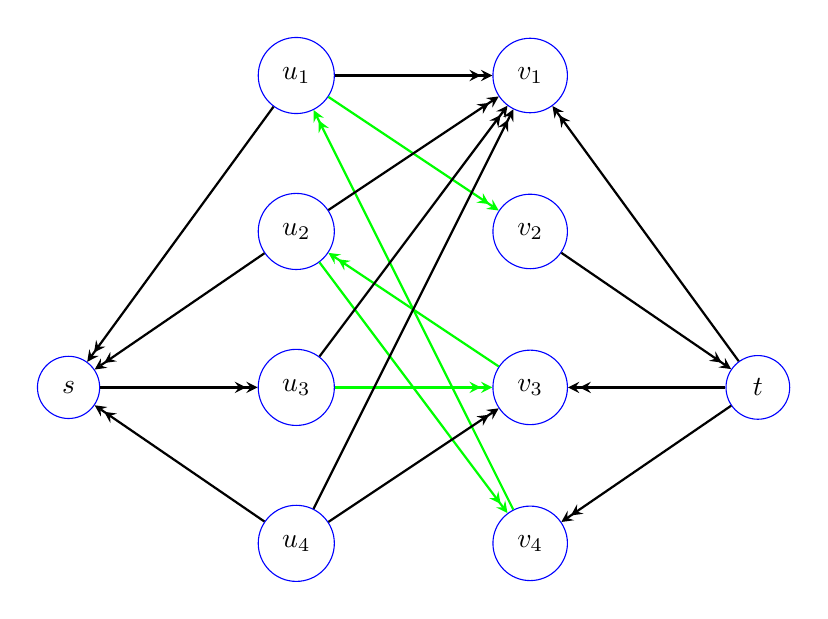
\begin{tikzpicture}[unmarked/.style={circle,inner sep=0.2cm,draw = blue}, edge/.style={thick,->>,>=stealth},blank/.style={},alternate/.style={thick,->>,draw=green,>=stealth}]
\matrix[row sep=1.0cm,column sep=2.0cm] 
{
\node()[blank]{};  \pgfmatrixnextcell \node(u1)[unmarked]{$u_1$};  \pgfmatrixnextcell \node(v1)[unmarked]{$v_1$};  \pgfmatrixnextcell \node()[blank]{};\\
\node()[blank]{};  \pgfmatrixnextcell \node(u2)[unmarked]{$u_2$};  \pgfmatrixnextcell \node(v2)[unmarked]{$v_2$};  \pgfmatrixnextcell \node()[blank]{};\\
\node(s)[unmarked]{$s$};  \pgfmatrixnextcell \node(u3)[unmarked]{$u_3$};  \pgfmatrixnextcell \node(v3)[unmarked]{$v_3$};  \pgfmatrixnextcell \node(t)[unmarked]{$t$};\\
\node()[blank]{};  \pgfmatrixnextcell \node(u4)[unmarked]{$u_4$};  \pgfmatrixnextcell \node(v4)[unmarked]{$v_4$};  \pgfmatrixnextcell \node()[blank]{};\\
};

\draw [edge] (u1) to (v1);
\draw [alternate] (u1) to (v2);
\draw [alternate] (v4) to (u1);
\draw [edge] (u2) to (v1);
\draw [alternate] (v3) to (u2);
\draw [alternate] (u2) to (v4);
\draw [edge] (u3) to (v1);
\draw [alternate] (u3) to (v3);
\draw [edge] (u4) to (v1);
\draw [edge] (u4) to (v3);

\draw [edge] (u1) to (s);
\draw [edge] (u2) to (s);
\draw [edge] (s) to (u3);
\draw [edge] (u4) to (s);
\draw [edge] (t) to (v1);
\draw [edge] (v2) to (t);
\draw [edge] (t) to (v3);
\draw [edge] (t) to (v4);
\end{tikzpicture}
\end{enumerate}


\item Let $G=(U,V,E)$ be the bipartite graph whose $U$ set represents the set of children, and $V$ set represents the set of ice-cream flavors. The $(u,v)\in E$ iff child $u$ likes ice cream $v$.
The children rushing for their ice cream resulted in the matching  
\[M=\{(A,\mbox{Cher}),(C,\mbox{Choc}),(D,\mbox{MC}),(E,\mbox{RR})\}.\] The flow graph $F_{G.M}$ below shows an alternating
path $P$ (in green) for which 
\[M^{*}=P\oplus M=\{(A,\mbox{V}),(B,\mbox{Choc}),(C,\mbox{RR}),(D,\mbox{MC}),(E,\mbox{Cher})\}.\]

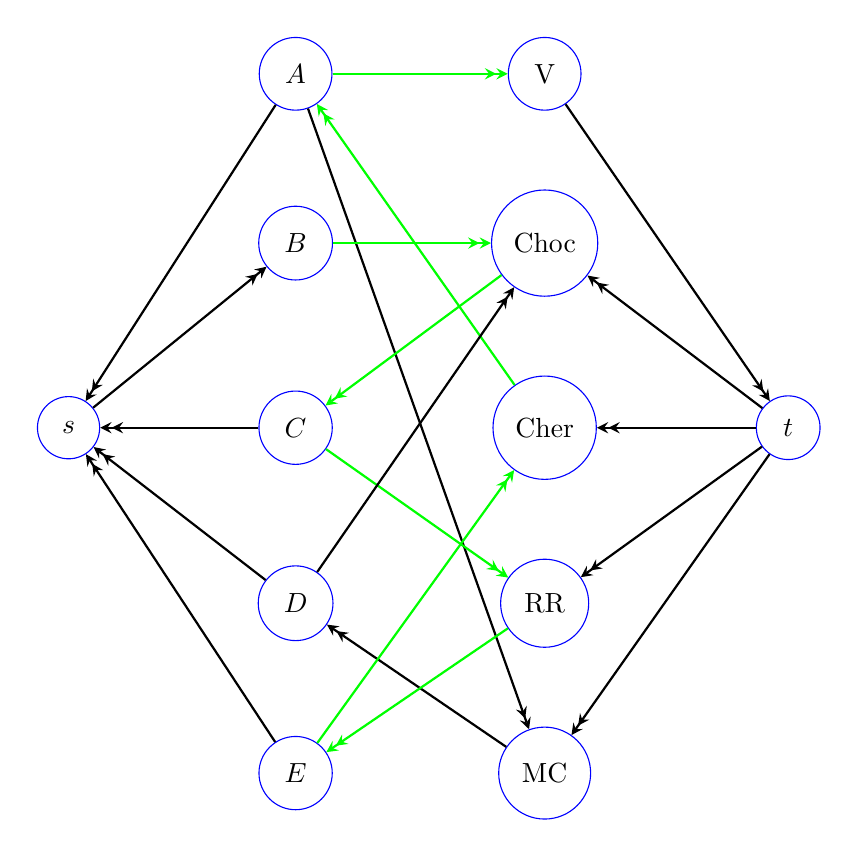
\begin{tikzpicture}[unmarked/.style={circle,inner sep=0.2cm,draw = blue}, edge/.style={thick,->>,>=stealth},blank/.style={},alternate/.style={thick,->>,draw=green,>=stealth}]
\matrix[row sep=1.0cm,column sep=2.0cm] 
{
\node()[blank]{};  \pgfmatrixnextcell \node(A)[unmarked]{$A$};  \pgfmatrixnextcell \node(V)[unmarked]{\mbox{V}};  \pgfmatrixnextcell \node()[blank]{};\\
\node()[blank]{};  \pgfmatrixnextcell \node(B)[unmarked]{$B$};  \pgfmatrixnextcell \node(Choc)[unmarked]{\mbox{Choc}};  \pgfmatrixnextcell \node()[blank]{};\\
\node(s)[unmarked]{$s$};  \pgfmatrixnextcell \node(C)[unmarked]{$C$};  \pgfmatrixnextcell \node(Cher)[unmarked]{\mbox{Cher}};  \pgfmatrixnextcell \node(t)[unmarked]{$t$};\\
\node()[blank]{};  \pgfmatrixnextcell \node(D)[unmarked]{$D$};  \pgfmatrixnextcell \node(RR)[unmarked]{\mbox{RR}};  \pgfmatrixnextcell \node()[blank]{};\\
\node()[blank]{};  \pgfmatrixnextcell \node(E)[unmarked]{$E$};  \pgfmatrixnextcell \node(MC)[unmarked]{\mbox{MC}};  \pgfmatrixnextcell \node()[blank]{};\\
};

\draw [alternate] (A) to (V);
\draw [alternate] (Cher) to (A);
\draw [edge] (A) to (MC);
\draw [alternate] (B) to (Choc);
\draw [alternate] (Choc) to (C);
\draw [alternate] (C) to (RR);
\draw [edge] (D) to (Choc);
\draw [edge] (MC) to (D);
\draw [alternate] (E) to (Cher);
\draw [alternate] (RR) to (E);
\draw [edge] (A) to (s);
\draw [edge] (s) to (B);
\draw [edge] (C) to (s);
\draw [edge] (D) to (s);
\draw [edge] (E) to (s);
\draw [edge] (V) to (t);
\draw [edge] (t) to (Choc);
\draw [edge] (t) to (Cher);
\draw [edge] (t) to (RR);
\draw [edge] (t) to (MC);
\end{tikzpicture}

\item Let $A$, $B$, and $C$ be sets. Assume $x\in A\oplus B$. Without loss of generality, assume $x\in A$ and $x\not\in B$.

\textbf{Case 1:} $x\in C$. Then $x\in B\oplus C$. 

\textbf{Case 2:} $x\not\in C$. Then $x\in A\oplus C$. 

It follows that $A\oplus B\subset (A\oplus C)\cup (B\oplus C)$. Therefore,
\[|A\oplus B|\leq |(A\oplus C)\cup (B\oplus C)|\leq |(A\oplus C| + |B\oplus C|.\]



\end{enumerate}



\end{document}






	
